\begin{savequote}
    \qauthor{\LARGE{Ville Sundell}}
\end{savequote}
\chapter{A utilization of Jabber Instant Messaging}
\label{c:jim_client_server}


\section{Introduction}
\label{s:jim_client_server:introduction}

I here pass on a message about open and free protocols and server-side freedom,
especially focussing upon instant messaging. The point of this article is to
help users utilize \textit{Jabber/XMPP} – the free and open instant messaging
protocol suite, and free software implementations of it.

Alongside an analysis of open and proprietary services, this paper is also meant
to be an easy guide to Jabber, which a system administrator could hand to users.


\section{A brief history of personal Internet Instant Messaging}
\label{s:jim_client_server:history}

The invention which is said to start the era of Internet instant messaging was
\textit{IRC}, originally an ASCII-based protocol and server software, initially
developed by F\hbox{}innish student Jarkko Oikarinen in 1988.

When a user connect to an IRC network (which consists of one or more server
machines), the user is  using only that particular network and the chat rooms
and users are available only in that network. So, if a user wants to chat in a
room which is not in the current network or wants to talk to friends not
available in the current network, another connection has to be created to
\textit{another} network (which is like a completely dif\hbox{}ferent universe
with dif\hbox{}ferent services and dif\hbox{}ferent users).

As time passed by the problems of centralized IM services became more visible,
eventually in 1998 spawning Jabber, the decentralized and open XML-based
protocol.  The centralized model was very convenient for big companies like AOL,
Yahoo and Microsoft, because now they could provide free IM services for users
of their other services (Email, Software suite, etc.). For these companies, it
was very convenient to get people to use only one network, one protocol and one
client. With this model, they got more users for their other software and
increased their market share, and got income mostly from selling advertisements
which would be shown in the client program.

So, combining instant messaging with other software, those large vendors were
able to get a really strong and prof\hbox{}itable position in the f\hbox{}ield
of personal IM.  The model worked well for several years for both customers and
vendors. However, now, after year 2000, mostly because of a larger user base,
the problems which computer-oriented people had seen for a decade with this
model, started to show up for normal users\ldots


\section{Problems with centralized and non-free solutions}
\label{s:jim_client_server:problems_centralized}

It seems, that now, from the end users' point of view, the current non-free
instant messaging protocols and implementations, like \textit{MSN} or
\textit{AOL} are working f\hbox{}ine: users can connect with a wide variety of
dif\hbox{}ferent clients. They can message their friends, and everything just
works.  However, the f\hbox{}irst signs of a collapse of proprietary IM systems
were evident during the last few years: client's advertisements becoming more
and more visible, censorship and manipulation of user's messages, increased
downtime, and sudden protocol changes are disturbing the communications of the
end user.

Usually, in normal and healthy customer-vendor relationship, the customer is
free to change the vendor if that vendor is not delivering the goods the
customer ordered, or the vendor is having bad problems when delivering them.
This fair competition setup should help vendors automatically improve the
quality of services. Well, that is how it should work in the perfect world.
However,  the situation we are talking about here is called ``vendor lock-in'',
a situation where the customer (here a customer is the user of the IM service)
is ``locked'', to a certain vendor (here, a vendor is a provider of an IM
service), without the possibility of changing the vendor itself.

In IM world, this ``lock-in'' is archived by a very familiar factor: the users!
Usually, the biggest reason for people  not wanting to change the vendor is that
the people they want to be in contact with are using the same service, but are
not available in the service you would like to use. So, because everyone uses
their own protocol, users from MSN can't communicate with users using Yahoo's
services. And, as we know, communicating with other people is the main purpose
of IM, right?

So, we are in a situation where the technical features of the protocol, quality
of client software, features of the network and small downtime, are not good
enough reasons to change, in the end-users' point of view. This might lead us to
think, if users are happy and can live with these problems, is the change really
worth it?


\section{Dangers of proprietary IM services}
\label{s:jim_client_server:dangers_proprietary}

Although the problems mentioned above do not seem to be critical enough to force
the change of an IM service provider, that is only because we do not seem to see
yet where this road is leading us. 

In our present time, we can already see some of the problems. Next, let's
discuss what those are, how we can see them, and where all this is leading in
the near future.


\subsection{Censorship and message manipulation}
\label{ss:jim_client_server:dangers_proprietary:censorship}

In the beginning of August 2007, a bunch of people started to track a problem
with MSN, which seemed like a server error: some messages didn't get through.
However, it was noted that those messages which didn't get through had some URLs
in them. More precisely, every message which had some URLs using a top level
domain ``.info'' \textit{(e.g. ``http://www.example.info'')}, got automatically
blocked. The news started to spread in the Internet, and people looked for more
keywords which would be also blocked.

It turned out that there were plenty of them, all involving URLs somehow. The
of\hbox{}f\hbox{}icial response from Microsoft was that the URL blocking was
part of their anti-virus war, and it was needed for that reason. And, all of
this, is legal (because usually a service provider can decide, what to pass and
what not to).  At the time of writing, it seems that you can send normal
``.info'' URLs, but still the service seems to block messages like
\textit{``http://www.example.info/download.php''} (\textit{``download.php''} is
also one of the magic keywords).

AOL and \textit{ICQ} are also blocking certain messages, but in their services
usually only HTML-tags which can be used for inserting scripts in the clients'
end are blocked.

Because the blocking is at the server-side, there is nothing we can do in the
user side (except use a service like
Tinyurl\footnote{\url{http://ur1.ca/f6pa}}, but that is not really solving
the problem, it just rounds it). Because the servers are operated by one entity,
it can freely decide what kind of messages it wants to forward to the users. So
in this situation, switching to an alternative client is not helping us.
However, in the next situation, it does help.


\subsection{Advertisements}
\label{ss:jim_client_server:dangers_proprietary:advertisements}

As probably every user of large IM services knows already, the
of\hbox{}f\hbox{}icial clients (like MSN Messenger and Yahoo! Messenger) are
nowadays fully loaded with all kinds of advertisements, which can be based on
text, still or animated images, and even audio.

But, unlike the previous problem, this can be rounded (so far), by switching to
alternative clients, which usually are free and open source (e.g.
\textit{Pidgin}\footnote{\url{http://ur1.ca/f6pc}}), but that will lead us to
the other problem, which we discuss next.


\subsection{Protocol changes}
\label{ss:jim_client_server:dangers_proprietary:protocol_changes}

Sometimes it can happen that a service provider suddenly changes the networking
protocol, so that current alternative clients are not able to connect to the
network any more without modif\hbox{}ications to the client code. With MSN this
happened in 2008, when it suddenly leapt to a new protocol version. This led to
a situation where the current alternative clients didn't work any more, and
needed an update from the vendor.


\subsection{Downtime}
\label{ss:jim_client_server:dangers_proprietary:downtime}

With centralized solutions, the downtimes are a big problem for the quality of
the service because, if the centralized servers go down (suf\hbox{}fering from
bugs, security holes, high network load or broken connections), there is, of
course no way to use the service.


\subsection{Diversity}
\label{ss:jim_client_server:dangers_proprietary:diversity}

Usually, in software development, diversity is sometimes considered a good
factor which breeds new innovations. But when this concept is applied to
networking protocols, the result is a mess. As we know, there is no way to
connect AOL users directly from an MSN network. In small countries, where one
protocol acts as the major protocol (usually, one country has one dominating
protocol, but the protocol changes from country to country), the diversity is
not a very visible problem. But when trying to contact friends from another
country, that may require using a dif\hbox{}ferent service.

 
\subsection{Seeing beyond the IM}
\label{ss:jim_client_server:dangers_proprietary:beyond_im}

One thing which proprietary IM services seem to miss, is thinking of the
communication beyond normal text/voice/video messaging. Usually, because of
restricted design, this is not possible to implement easily.

With free and open protocols (like Jabber/XMPP), users can use the basic
protocol to transmit their own data; for example, for your own application.

There are already tons of extensions for the basic XMPP protocol, but there are
more and more coming all the time. For example the upcoming \textit{Google Wave}
will be based on XMPP (which is not only about instant messaging).


\section{So, what is this Jabber?}
\label{s:jim_client_server:what_is_jabber}

The answer is simple: the solution. Basically Jabber is a free decentralized
solution for communication between two or more users. There are no central
servers, rather there are many providers of the service. These providers
communicate between their users and other Jabber providers. Becoming a provider
is easy, you just need a machine to run some Jabber server (which we will
discuss later). Becoming a user of Jabber is way more easy, you need just a
client, and a server to connect. We will discuss it in the next chapter.

In a technical point of view, Jabber is a combination of XML-based XMPP-base
protocol and extensions to that protocol (called XEPS, also based on XML).

The XMPP protocol can handle most basic tasks, like authentication,
encryption, sending and receiving data to dif\hbox{}ferent users, and
server-to-server connections. Both XMPP and XEPs are managed by the XMPP
Standards Foundation (XSF), but users are still free to create their own
extensions to the protocol.

Most important XEPs include:
\begin{itemize}
    \item{MUC – multi user chats (``chatrooms'')}
    \item{User prof\hbox{}iles}
    \item{XHTML messages}
\end{itemize}

Now you know the basics about Jabber and XMPP, so let's start using Jabber,
learning more about Jabber as we advance.


\section{Using Jabber}
\label{s:jim_client_server:using_jabber}


\subsection{The F\hbox{}irst step – becoming a ``Jabberist''}
\label{ss:jim_client_server:using_jabber:the_first_step}

The only thing you really need is a client. Here is listed a few good
free-software clients:
\begin{itemize}
    \item{Pidgin (it can handle many protocols, like MSN and IRC, in addition to
        XMPP/Jabber, multiplatform)}
    \item{Psi (Only Jabber)}
    \item{Miranda (Windows only)}
\end{itemize}

After you have selected the client (I use Pidgin, it also comes pre-installed in
Ubuntu and other modern free-software-based operating systems), and installed
it, now it is time to f\hbox{}ire it up, and create a new account.

\begin{wrapfigure}{l}{0mm}
    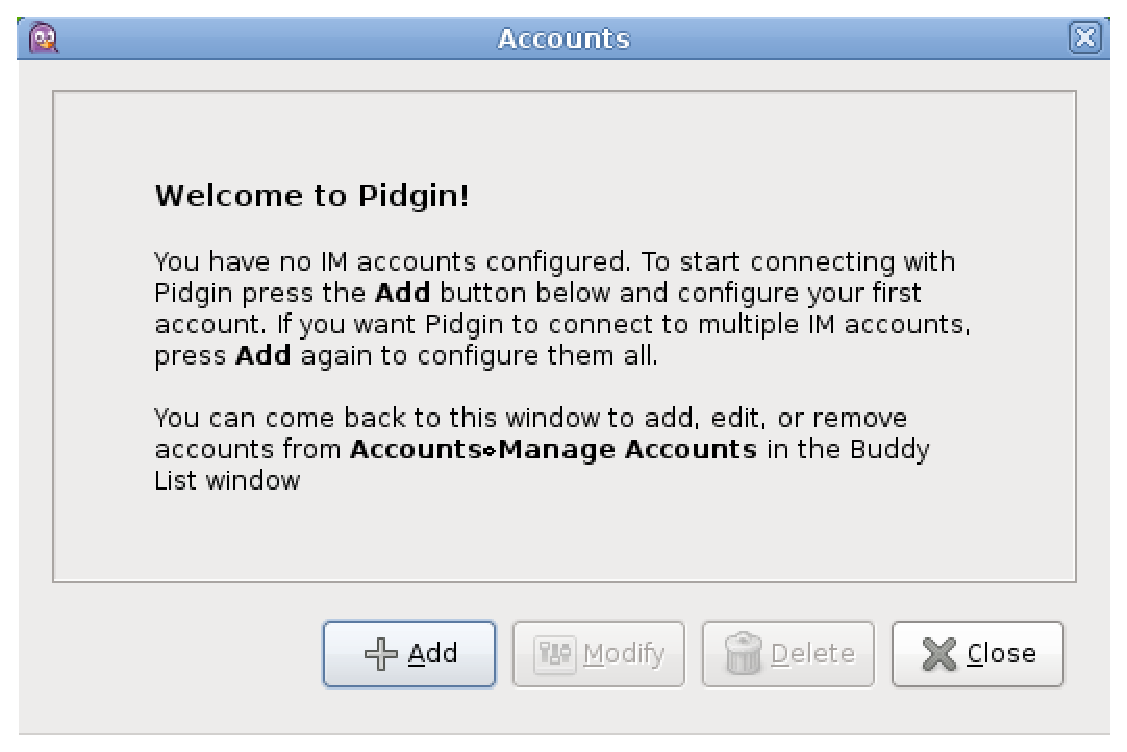
\includegraphics[scale=0.40]{./media/jabber_pidgin_accounts}
\end{wrapfigure}

Here we are working with Pidgin, but  the same f\hbox{}ields mostly exist in
other clients.

F\hbox{}irst, when you start up Pidgin, you will see this:

You will see the dialogue pictured here only at f\hbox{}irst startup, when there
are no other accounts. Here, just hit ``Add'' to see next dialogue, and add the
f\hbox{}irst account.

\begin{wrapfigure}{l}{0mm}
    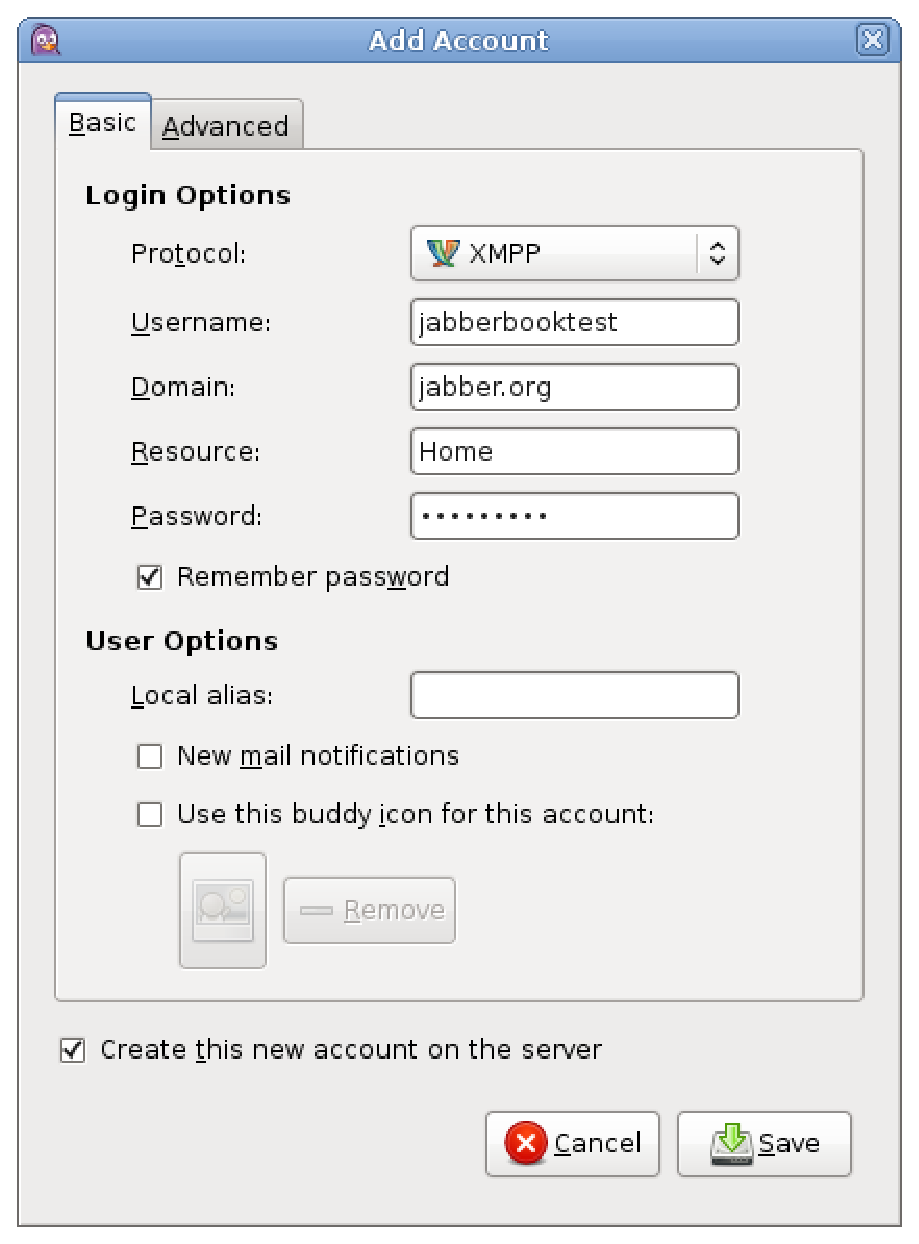
\includegraphics[scale=0.40]{./media/jabber_pidgin_add_account}
\end{wrapfigure}

Just f\hbox{}ill the dialogue in as it is shown. You usually don't need to care
about the options of the Advanced-tab, usually they are right. But if you are
experiencing some network problems, you should check that tab also. The only
things which vary here are your ``Username'' and ``Password'' f\hbox{}ields.
Change these according to your wishes, otherwise everything should be alright. 

``Domain'' is the server, where do you want to save your account, jabber.org is
general server, which is open for everyone.

``Resource'' is free-form string, which tells the location where you are
connecting.

If you are the only person using this account, it is safe to check the
``Remember password'' box.

Check also the last box, to be able to register your account, if you are
creating a new account (if this is your f\hbox{}irst time, you are creating a
new account, so you can check this box). Otherwise, if you know your account
exists on the server already, and you are just connecting to that account
normally, do not check this box.

Next, after clicking the ``Save'' button, you will need to wait a bit, and you
should see this kind of dialogue:

\begin{wrapfigure}{l}{0mm}
    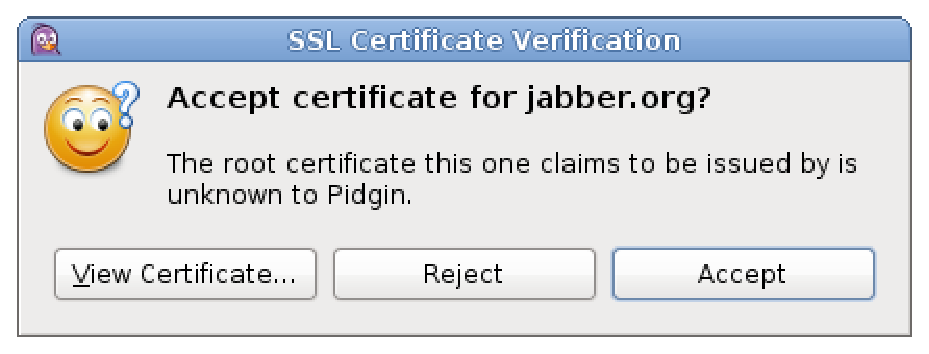
\includegraphics[scale=0.40]{./media/jabber_pidgin_ssl_certificate_verification}
\end{wrapfigure}

This means, that the server is using a so-called self signed certif\hbox{}icate.
If you want, you can view detailed information about the certif\hbox{}icate by
clicking the ``View Certif\hbox{}icate\ldots'' button. The checksum of the
certif\hbox{}icate should be
\textbf{e8:b8:c4:f2:41:5f:fb:64:9f:5d:be:52:1c:da:8f:a6:a4:fc:33:6e}, this will
expire Thu Dec 17 19:56:18 2009, so after that, the checksum is going to change.
But in most cases, the certif\hbox{}icate should be f\hbox{}ine, so you can just
click “Accept”.  After this initial acceptance, in future, if your client
complains about the certif\hbox{}icate not being valid, you have to take that
seriously, because it can be that you are under a DNS spoof\hbox{}ing attack.

Anyway, presuming that noone is going to attack you, and that the sky is not
falling on your head, press ``Accept'', and f\hbox{}ill up this dialogue:

\begin{wrapfigure}{l}{0mm}
    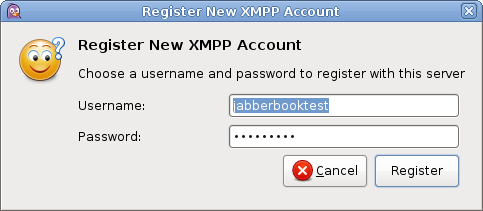
\includegraphics[scale=0.40]{./media/jabber_pidgin_register_new_xmpp_account}
\end{wrapfigure}

This is now a conf\hbox{}irmation about the account you are going to create to
the server. This is exactly the same information you gave in the ``Add Account''
dialog above, so you can just hit ``Register'', and move to the next dialogue.

If registration is not successful, check the information you gave to Pidgin, it
is possible that there is already someone using the username you wanted. In this
case, you have to select another username. After a successful registration you
should see a dialogue like this:

\begin{wrapfigure}{l}{0mm}
    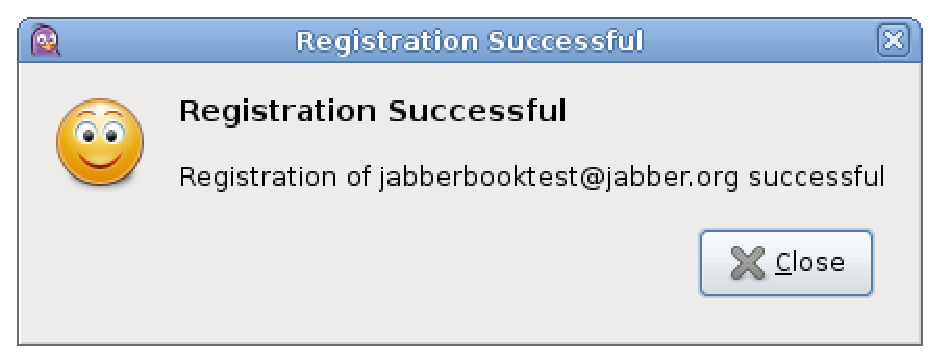
\includegraphics[scale=0.40]{./media/jabber_pidgin_registration_successful}
\end{wrapfigure}

Congratulations, now you have your f\hbox{}irst Jabber account!
	
There is just one more step, in the following dialogue, check the ``Enabled''
box for your account like this:

\begin{wrapfigure}{l}{0mm}
    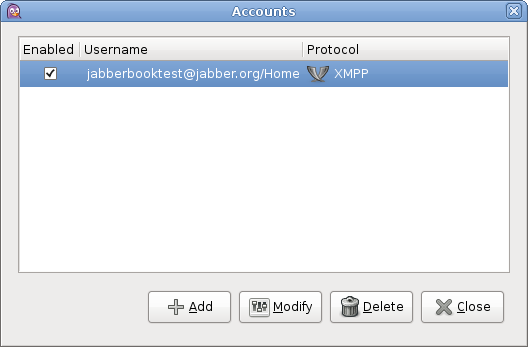
\includegraphics[scale=0.40]{./media/jabber_pidgin_accounts_2}
\end{wrapfigure}

And the Pidgin connects to the server!


\subsection{More advanced use of Jabber: Sending messages}
\label{ss:jim_client_server:using_jabber:advanced_use}

You can now send messages to individual people just by clicking the ``Buddies''
menu at the top of the  ``Buddy List'' window and select ``New instant
message''. After that, if you have many accounts connected, select the right
account from the popup menu, and then just write the Jabber ID \textit{(JID)} of
the person you want to message with. When pressing OK, new window (or if you
already have an IM window, it will create a new tab), and there you can send
messages to the person.


\section{End words}
\label{s:jim_client_server:end_words}

I hope that from this article users have been able to see the basic need for
free and open, decentralized instant messaging solutions, and become familiar
with the basics of Jabber/XMPP.





